\documentclass{report}

\usepackage[utf8]{inputenc}  % Ng Edit for accents in Spanish
\usepackage[spanish]{babel}  % Ng Edit for accents in Spanish
\usepackage{hyperref}        % Ng Edit for adding urls
\usepackage{graphicx}        % Ng Edit for adding graphics

%Path relative to the .tex file containing the \includegraphics command
\graphicspath{ {img/} }

\def\equationautorefname~#1\null{(#1)\null} %to use parenthesis in eqs.

\title{\bf
  Mejora en la asignación de recursos con Particle Swarm Optimization para el
  control de enfermedades transmitidas por mosquitos
}

\author{Topiltzin Hernández Mares}

\begin{document}

\maketitle
\thispagestyle{empty}
\pagestyle{empty}
\tableofcontents
\listoffigures

\begin{abstract}
\end{abstract}

\chapter{Introducción}

\chapter{Estado del arte}
  Antes de hablar del problema y su solución, es necesario entrar en contexto.
  Por esto, en la primera sección de este capítulo se definirán conceptos
  básicos, tales como trampas para mosquitos, las cuales tienen un papel central
  en el problema. Enseguida, se hablará sobre términos de inteligencia
  artificial y métodos de optimización, los cuales ayudarán a entender mejor las
  problemática y su solución.
  
  En la segunda parte de este capítulo se hablará de algunos trabajos recientes
  para poder entender el estado del arte en problemas de optimización. Sin
  embargo, por la poca investigación relacionada a la optimización de vigilancia
  de mosquitos, se analizarán trabajos similares enfocados en redes y
  monitoreo.

\section{Conceptos básicos}
  \subsection{Inteligencia artificial}
    En el libro Artificial Intelligence: A Modern Approach
    \cite{AIModernAproach}, se define la inteligencia artificial (IA) como
    máquinas con pensamiento parecido al humano y con acciones racionales.
    
    Una definición más elaborada es la de \cite{AIDef}: IA es un término
    utilizado para etiquetar a computadoras que imitan funciones humanas
    cognitivas, tales como aprendizaje y resolución de problemas. De igual
    manera, se llama inteligencia artificial a algoritmos que trabajan con la
    misma complejidad que expertos humanos.
  
  \subsection{Optimización}
    Puede ser definida como el proceso de encontrar la mejor solución posible
    entre todas las disponibles. Por lo tanto, la tarea de optimización es
    modelar algún problema en términos de alguna función de evaluación y emplear
    algún algoritmo de búsqueda para minimizar (o maximizar) esa función
    objetivo. Sin embargo, no es posible asegurar que el resultado óptimo será
    encontrado, ya que hay problemas demasiado grandes que es imposible
    encontrar la solución óptima \cite{SearchMethodologies}.
  
  \subsection{Heurísticas}
    En el área computacional de optimización, se llaman heurísticas a los
    métodos usados para buscar soluciones de alta calidad, sin asegurar la
    óptima.

    Una definición más elaborada la da \cite{HeuristicDef}, pues dice
    que una técnica heurística es un método que busca soluciones buenas (y casi
    óptimas) con un costo computacional bajo. Sin embargo, estos métodos no son
    capaces de indicar qué tan cerca de la optimización perfecta se encuentra 
    la respuesta actual dada por una heurística.
  
  \subsection{Metaheurísticas}
    Se refiere a técnicas que coordinan, manipulan y guían el comportamiento y
    soluciones de métodos heurísticos de optimización. Tales métodos pueden ser
    desde procedimientos de alto nivel o pueden describir las alteraciones
    posibles para una heurística \cite{MetaheuristicsDef}.

    Existe una gran cantidad de metaheurísticas
    \cite{HeuristicDef, SearchMethodologies}, más adelante se hablará de algunos
    métodos, tal como algoritmos genéticos y optimización de enjambre de
    partículas.
  
  \subsection{Inteligencia de enjambre}
    La inteligencia de enjambre es un campo computacional que diseña y estudia
    algoritmos para buscar soluciones a problemas. Estos algoritmos están 
    inspirados en el comportamiento complejo y, algunas veces, coordinado de
    enjambres de cualquier organismo natural \cite{SearchMethodologies}. 
    
    \begin{figure}[h]
      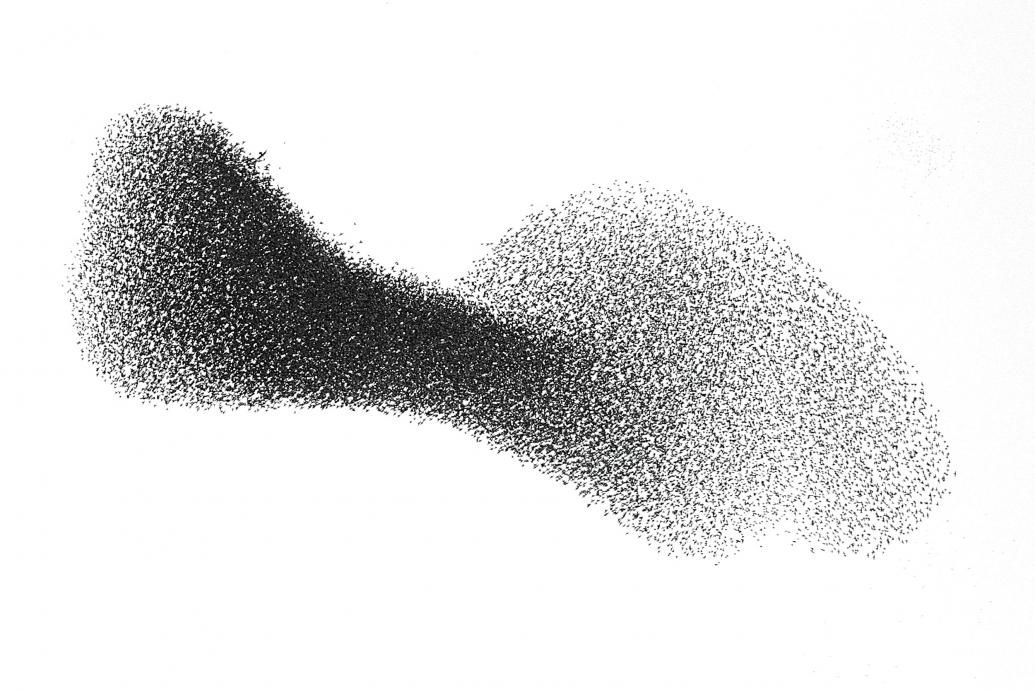
\includegraphics[scale=0.18]{si-repr}
      \centering
      \caption{Inspiración de algoritmos de inteligencia de enjambre.}
      \centering
    \end{figure}

  \subsection{Algoritmos evolutivos}
    Son un tipo de algoritmos que buscan soluciones a problemas, tomando
    inspiración de la selección natural y genética \cite{EADef,GADef}. Estos 
    algoritmos pueden representar cromosomas como cadenas de texto, los cuales 
    son las soluciones a los problemas; los alfabetos representan genes; y más
    conceptos tomados de la biología.

  \subsection{Particle Swarm Optimization}
    Particle Swarm Optimization (PSO) fue inventada por Eberhart y Kennedy en
    1995 \cite{PSODef}, es un algoritmo
    estocástico inspirado en el comportamiento de una parvada de aves en busca
    de alimento. Cada partícula en el algoritmo, que representa una solución al
    problema, vuela en el espacio de búsqueda, actualizando su velocidad y su
    posición. La ecuación clásica para actualizar la velocidad de una partícula
    es \ref{eq:1} y para actualizar su posición es \ref{eq:2}.

    \begin{equation}
      \label{eq:1}
      v_ij = v_ij + c_1 rand()(p_ij - x_ij) + c_2 rand()(p_nj - x_ij)
    \end{equation}

    \begin{equation}
      \label{eq:2}
      x_ij = x_ij + v_ij
    \end{equation}

    Actualmente, el algoritmo PSO canónico (CPSO) o PSO con peso inercial
    (PSO-iw) es considerado como el PSO estándar \cite{CPSO,PSOReview}.
    En esta forma de PSO, se introduce una nueva variable $w$, modificando
    \ref{eq:1} a \ref{eq:3}. Esta nueva variable equilibra la búsqueda local y
    global de la solución.

    \begin{equation}
      \label{eq:3}
      v_ij = w v_ij + c_1 rand()(p_ij - x_ij) + c_2 rand()(p_nj - x_ij)
    \end{equation}

\section{Trabajos relevantes en el área}
  \subsection{Optimización de ubicación de una red de sensores inalámbricos en
    un taller inteligente}
    En 2018, Li et al \cite{3DAFAO} desarrollaron un nuevo algoritmo con el
    objetivo de optimizar la ubicación de nodos de una red de sensores
    inalámbricos (WSN) para minimizar el error de detección de objetos 3D en un
    taller de manufactura inteligente.
    
    Los autores tomaron inspiración del comportamiento de enjambres de moscas,
    e implementaron en algoritmo de 
    optimización de moscas (FOA). Sin embargo, este algoritmo presenta un
    comportamiento 2D, y su problema necesita un análisis en tres dimensiones.
    Por esto, introdujeron una nueva dimensión en la búsqueda de soluciones,
    resultando en el algoritmo es 3D-FOA. Como una alternativa, decidieron
    añadir una variable más a su algoritmo, un peso inercial variable,
    proveniente de PSO-iw, resultando en un nuevo algoritmo: 3D-AFOA.

    Al tener dos algoritmos capaces de optimizar los nodos de la red MSN,
    realizaron diversos experimentos para comparar dichos métodos. Inicialmente,
    establecieron la posición fija de 3 nodos de la red y un solo nodo objetivo
    a detectar en un taller simulado. Establecieron una población de 50 y 500
    como número máximo de generaciones en ambos algoritmos. En la figura
    \ref{fig:location-error-3d-foa-3d-afoa_1} se muestran los resultados
    obtenidos.

    \begin{figure}[ht]
      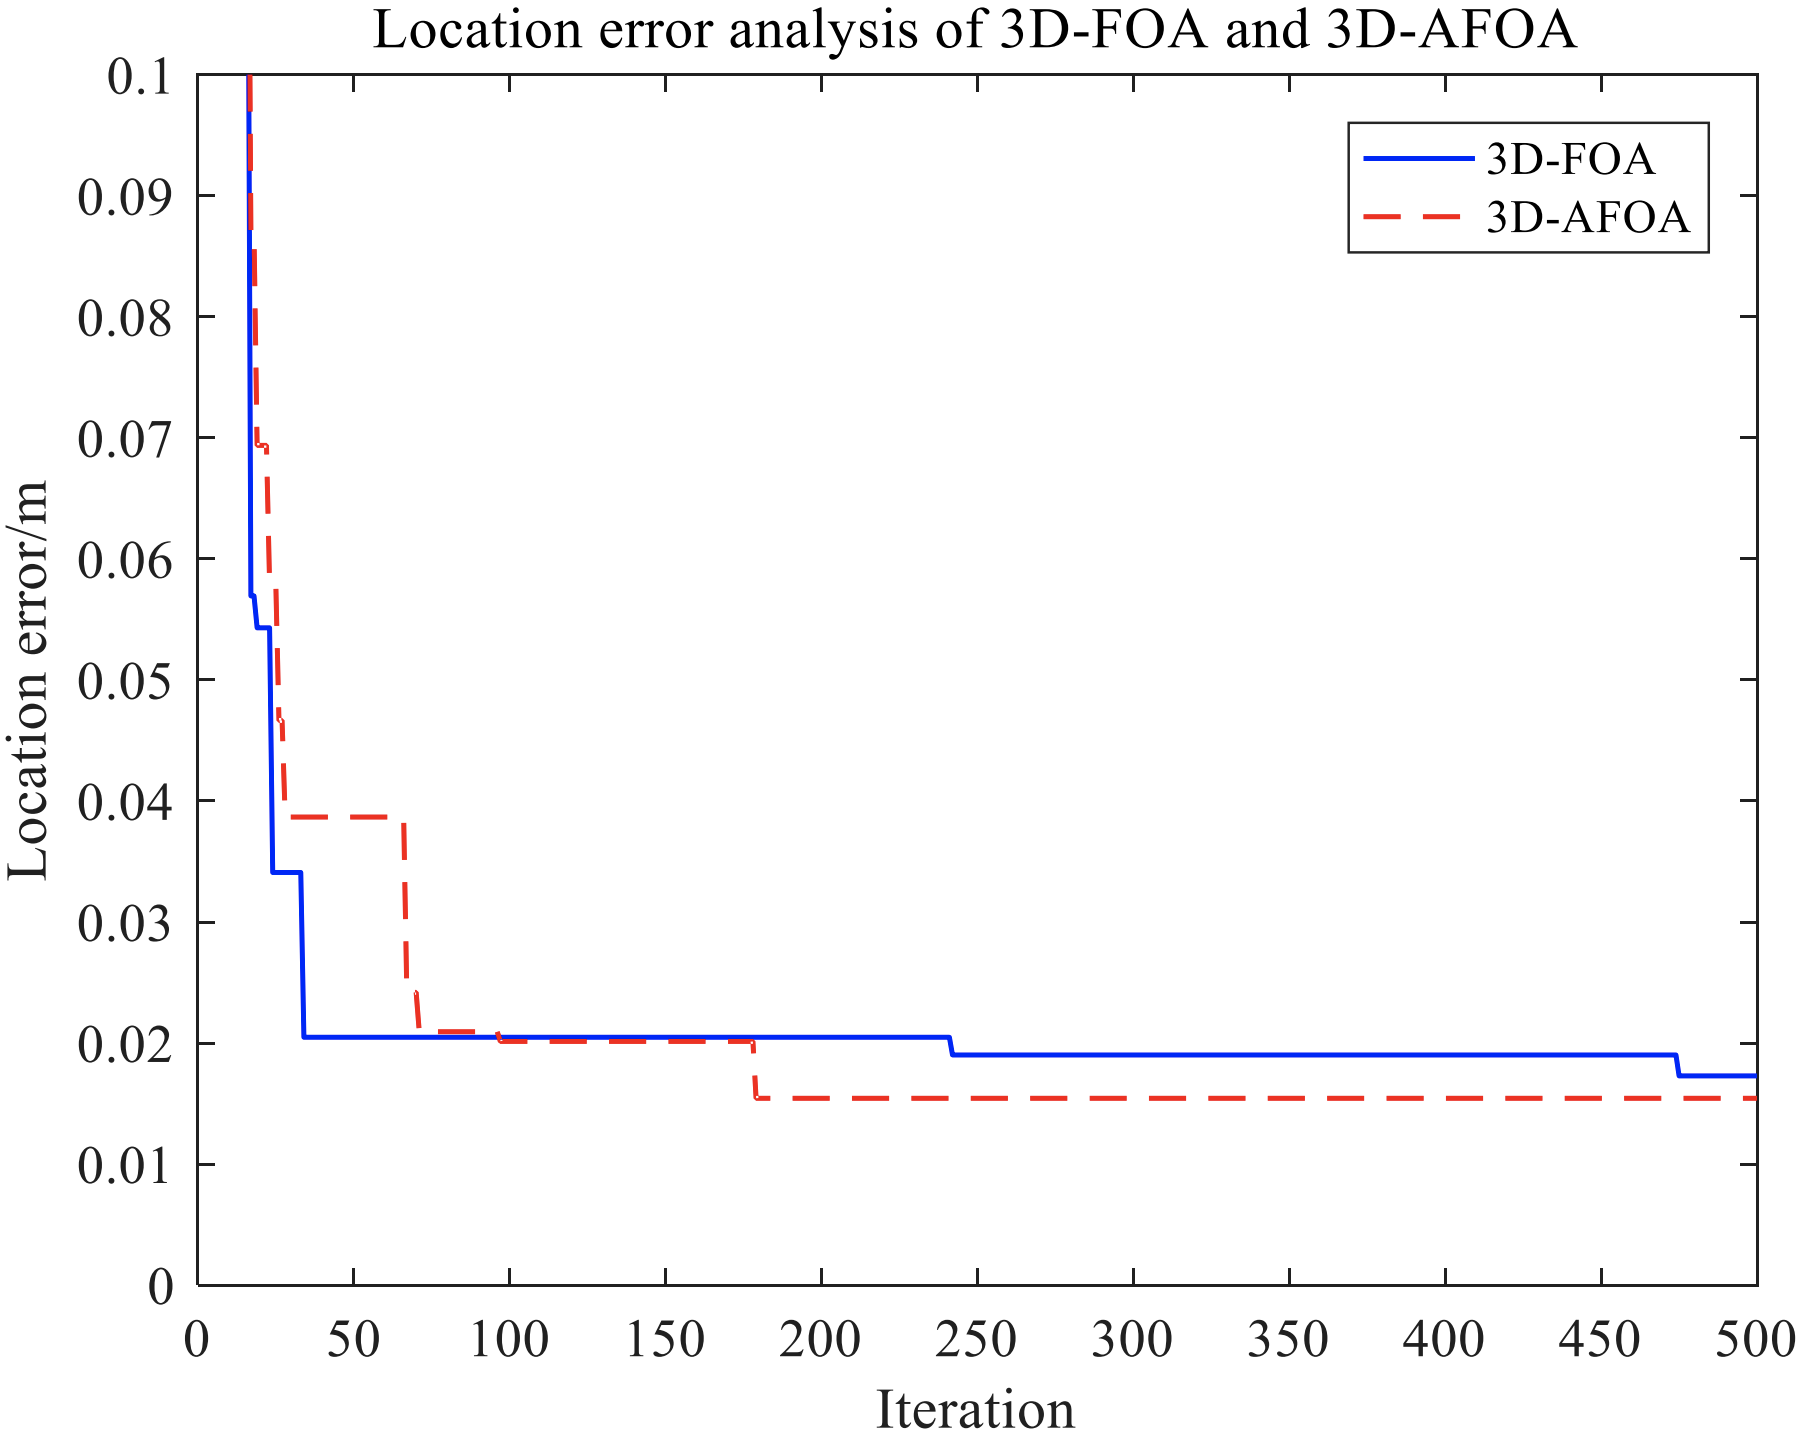
\includegraphics[width=\textwidth]{location-error-3d-foa-3d-afoa_1.png}
      \centering
      \caption{Resultados de error de detección de 3D-FOA y 3D-AFOA}
      \label{fig:location-error-3d-foa-3d-afoa_1}
      \centering
    \end{figure}

    Como se puede ver en la figura \ref{fig:location-error-3d-foa-3d-afoa_1}, el
    algoritmo 3D-AFOA tiene un mejor desempeño, pues converge en una mejor
    solución en menos generaciones. 

    Cone l objetivo de verificar la efectividad del algoritmo, se probó con 3, 4
    y 5 nodos fijos en la red para detectar nuevamente un recurso en el taller
    simulado. Los resultados se muestran en \ref{fig:location-error-3d-afoa_2}.

    \begin{figure}[ht]
      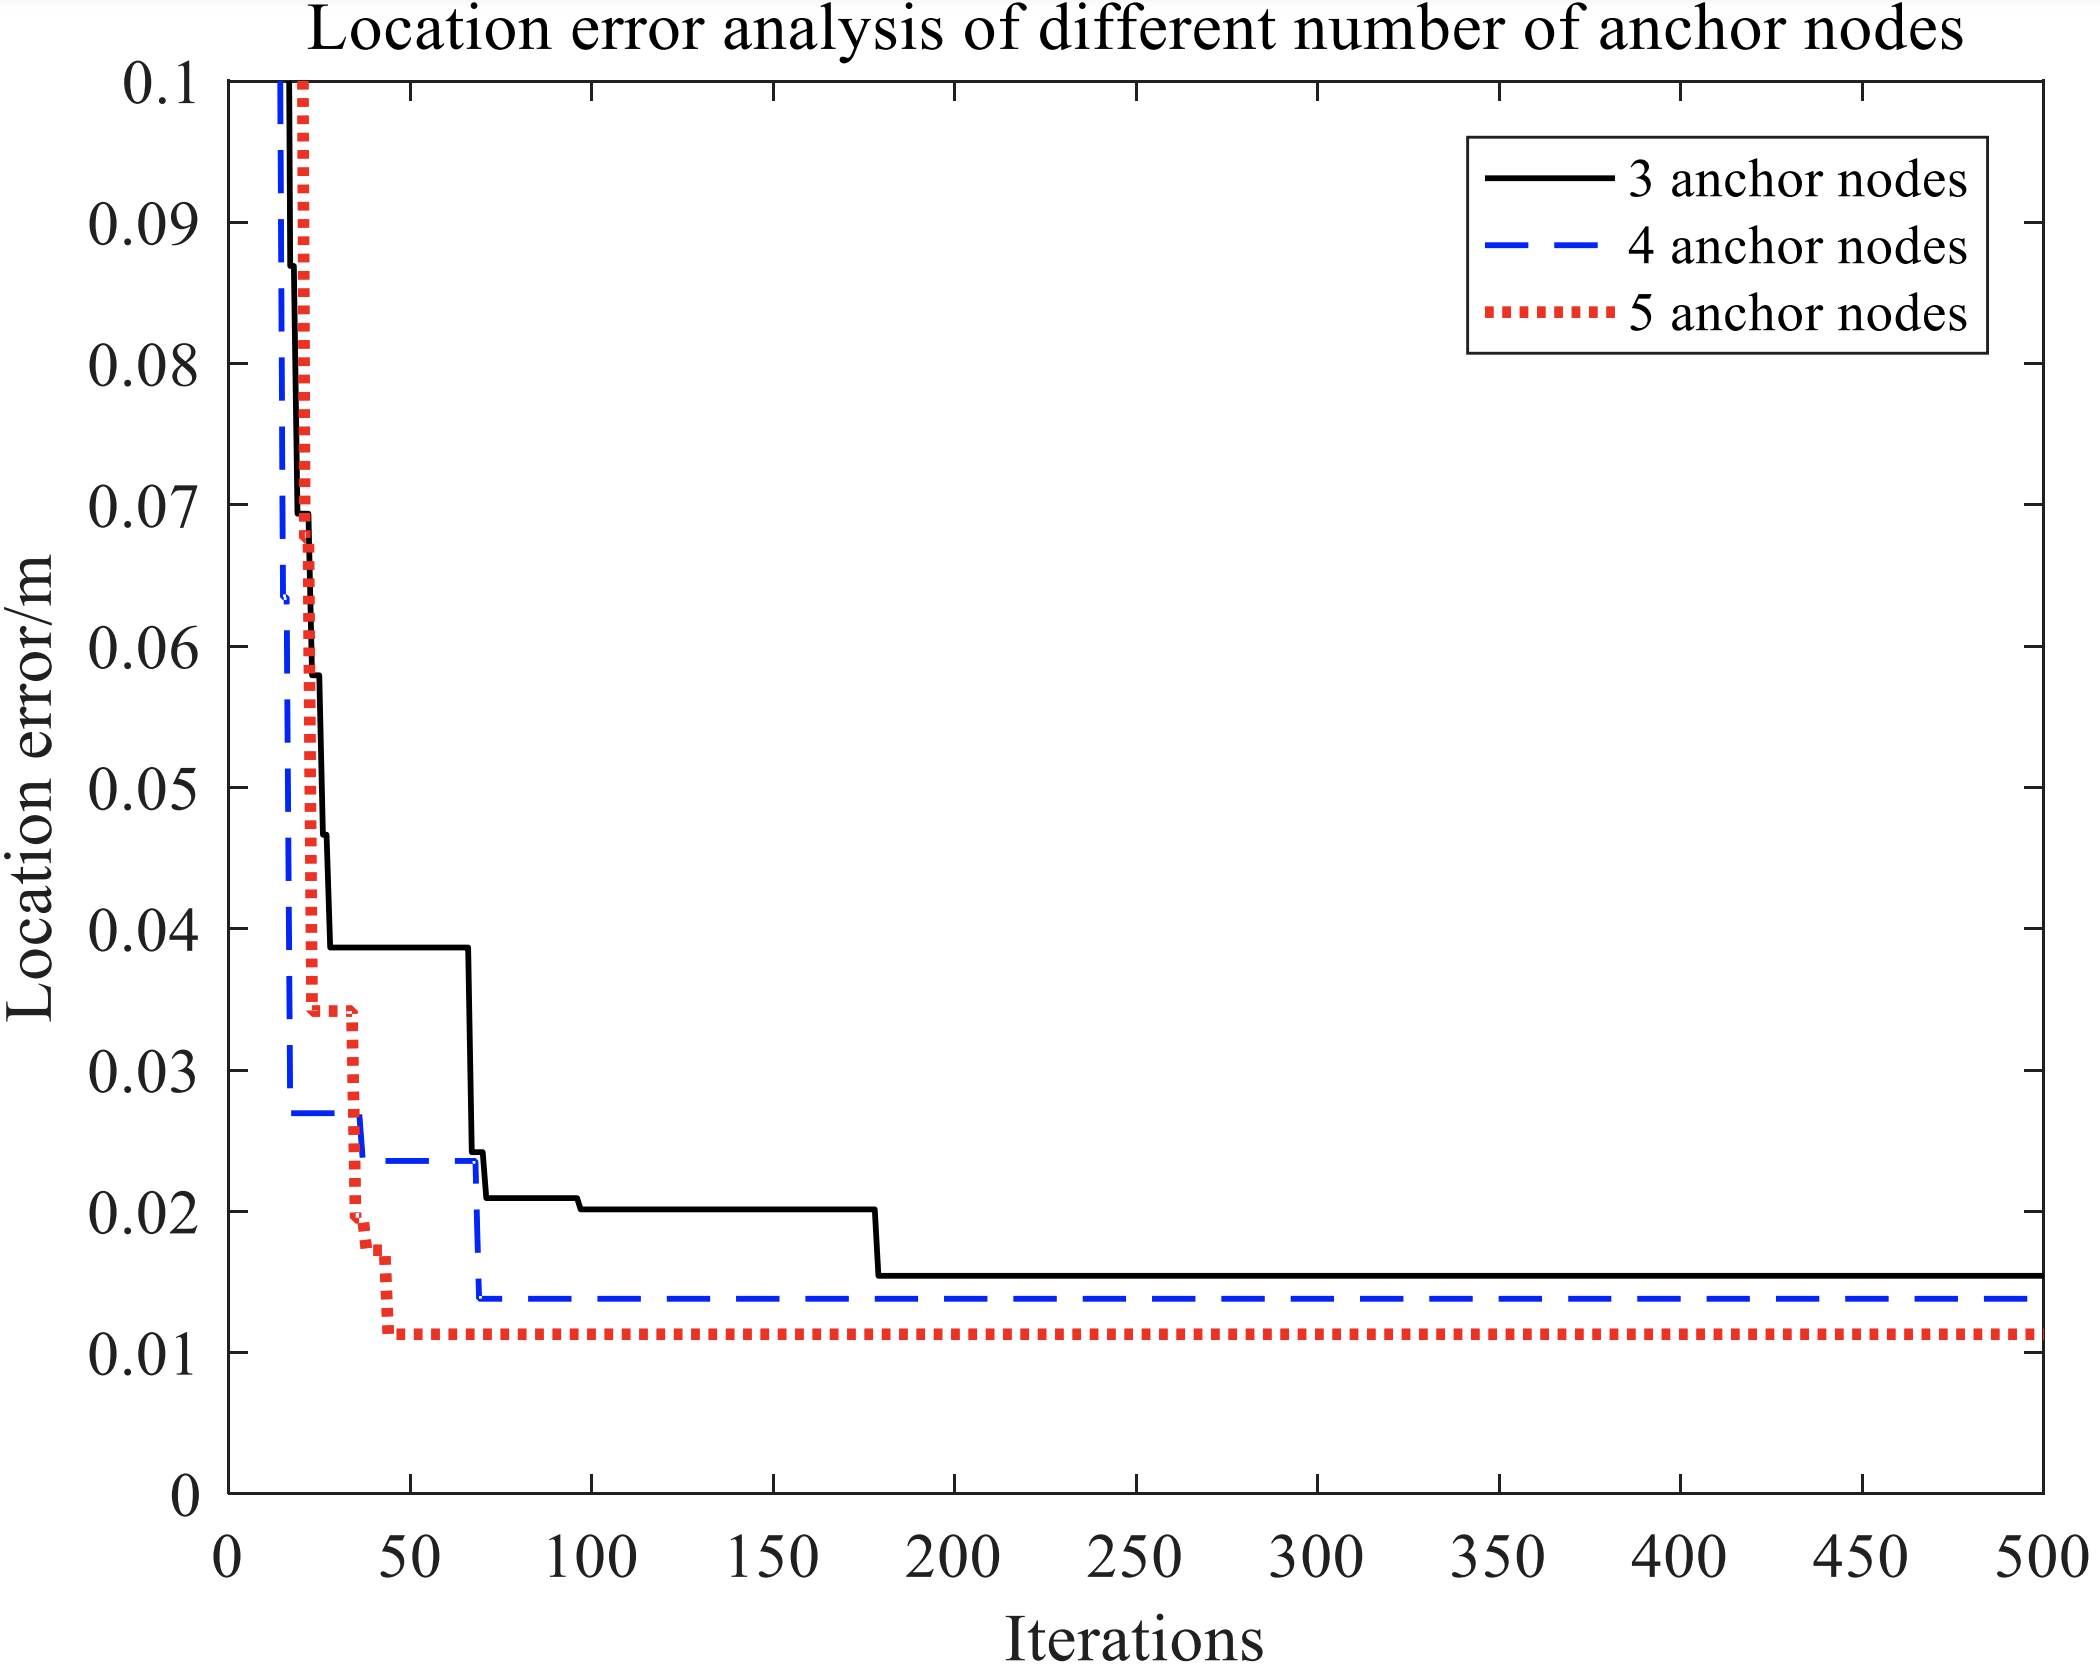
\includegraphics[width=\textwidth]{location-error-3d-afoa_2.png}
      \centering
      \caption{Resultados de error de detección con diferente cantidad de nodos}
      \label{fig:location-error-3d-afoa_2}
      \centering
    \end{figure}

    Analizando los resultados expuestos en \ref{fig:location-error-3d-afoa_2},
    se puede apreciar que, conforme incrementa el número de nodos en el
    algoritmo, el tiempo de convergencia acelera. Sin embargo, el
    error de detección de los objetivos, aunque mejora con más nodos, no existe
    gran diferencia. Esto es debido a que solamente la ubicación de un solo nodo
    fue optimizada en los algoritmos. 

    Para finalizar, los investigadores concluyeron que 3D-AFOA es altamente
    aplicable al problema de optimización en la ubicación de nodos en una red
    WSN y no requiere de un alto presupuesto computacional para lograr buenas
    soluciones. 

\section{Comparación}
\section{Conclusión}

\chapter{Problema y justificación}

\chapter{Solución}

\chapter{Metodología de evaluación}

\chapter{Resultados y contribuciones}

\chapter{Conclusiones}

\begin{thebibliography}{99}
  \bibitem{AIModernAproach}S. Russell and P. Norving, “Artificial Intelligence: A modern approach”, 3rd ed. Prentice Hall, New Jersey: Pearson Education, 2009. 
  \bibitem{AIDef}J. M. Spector and S. Ma, “Inquiry and critical thinking skills for the next generation: From Artificial Intelligence back to human intelligence,” Smart Learning Environments, vol. 6, no. 1, Sep. 2019. 
  \bibitem{SearchMethodologies}E. K. Burke and G. Kendall, “Search methodologies: Introductory tutorials in optimization and decision support techniques”. New York, New York: Springer, 2014.
  \bibitem{HeuristicDef}V. J. Rayward-Smith, “Modern Heuristic Search Methods”. Chichester, New York: Wiley, 1996. 
  \bibitem{MetaheuristicsDef}F. Glover and M. Laguna, “Tabu Search”. Boston, Massachusets: Kluwer Academic Publishers, 1997.
  \bibitem{EADef}C. A. Coello Coello, G. B. Lamont, and D. A. Van Veldhuizen, “Evolutionary algorithms for solving multi-objective problems,” Genetic and Evolutionary Computation Series, 2007. 
  \bibitem{GADef}A. S. Fraser, “Simulation of genetic systems by Automatic Digital Computers II. effects of linkage on rates of advance under selection,” Australian Journal of Biological Sciences, vol. 10, no. 4, p. 492, 1957. 
  \bibitem{PSODef}J. Kennedy and R. Eberhart, “Particle swarm optimization,” Proceedings of ICNN'95 - International Conference on Neural Networks, 1995. 
  \bibitem{CPSO}Y. Shi and R. Eberhart, “A modified particle swarm optimizer,” 1998 IEEE International Conference on Evolutionary Computation Proceedings. IEEE World Congress on Computational Intelligence (Cat. No.98TH8360), 1998. 
  \bibitem{PSOReview}S. Cheg, H. Lu, X. Lei, and Y. Shi, “A quarter century of particle swarm optimization,”, Complex and Intelligent Systems, vol. 4, no. 3, pp. 227 239, 2018.

  \bibitem{3DAFAO}S. Li, C. Zhang, and J. Qu, “Location optimization of wireless sensor network in Intelligent Workshop based on the three-dimensional adaptive fruit fly optimization algorithm,” International Journal of Online Engineering (iJOE), vol. 14, no. 11, p. 202, Nov. 2018. 
\end{thebibliography}

\end{document}
